\chapter{Técnologias}
\label{tecnologias}

\section{Javascript}
Javascript  é uma linguagem de programação interpretada, que foi criada com o intuito de ajudar os navegadores web a executar scripts no lado do cliente e assim permitir a interação com o usuário\cite{jsRight}. Esta linguagem foi baseada na ECMAScript\footnote{Que  é uma linguagem de programação de scripts.} que é padronizada pela Ecma international nas especificacões ECMA-262\footnote{\url{http://www.ecma-international.org/publications/files/ECMA-ST/Ecma-262.pdf}} e ISO/IEC 16262\footnote{\url{http://www.iso.org/iso/home/store/catalogue_tc/catalogue_detail.htm?csnumber=55755}}.
 \subsection{Imperativa e estruturada}
	
O Javascript possui elementos de sintaxe de linguagens de programação estruturada, elementos que se assemelham por exemplo com a linguagem C como “If”, “while”, “switch”.
Apesar de sintaticamente parecer com C, seu escopo é diferente, Javascript utiliza-se de um escopo á nível de função\footnote{Isso significa que somente funções podem criar novos escopos, blocos como if, while, for não criam novos escopos.}.


 \subsection{Tipagem dinâmica}
 
No Javascript os tipos são associados com valores e não com as variáveis. Por exemplo, uma variável "A" poderia ser associado a um número e posteriormente ser associado a uma string .

 

 \subsection{Baseada em objetos}

A linguagem Javascript possui suporte a  objetos, que são implementados como lista associativas. Os nomes da propriedade de um objeto  são strings e podem, junto com seus valores, ser adicionadas, mudadas ou deletadas em tempo de execução. Vale ressaltar que em Javascript existem alguns objetos padrões como “window” e “document”.


 \subsection{Baseada em protótipos}
 
 O Javascript utiliza-se de protótipos no lugar das classes para o mecanismo de herança. É possível simular muitas características de orientação a objetos usando-se de protótipos.

 \subsection{Linguagem dirigida e eventos}
 
 No Javascript é possível  tratar as interações do usuário em um arquivo HTML, e é através de eventos que isso é feito. Eventos provocados pela interação com o usuário podem ser desde  o clique de um botão do teclado até o envio de formulário, e a partir deles podemos criar diversas funções que são invocadas caso algum destes eventos aconteça.

 \subsection{Javascript X Java}

É muito comum as pessoas associarem Javascript com a linguagem Java por causa do nome, apesar de ambos terem java no nome, eles não possuem nenhuma relação. As principais diferença entre eles é que Java cria aplicações executadas em uma maquina virtual ou em um browser enquanto ao Javascript é executado apenas no browser. Códigos em Java precisam ser compilados enquanto que o Javascript é interpretada.


\section{MEAN Satck}
O nome MEAN é uma sigla que representa o conjunto de 4 ferramentas: MongoDB, Express.js, Angular.js e Node.js. Através deste conjunto de ferramentas podemos criar complexas aplicações web.
Existem algumas ferramentas que facilitam a utilização destas tecnologias em conjunto, automatizando algumas etapas para a criação de um projeto, alguns exemplos são o MEAN.js e MEAN.io, sendo que a diferença básica é a organização dos diretórios do projeto e alguns elementos extras que são adicionados ao MEAN para facilitar o desenvolvimento, por exemplo o MEAN.JS possui o YEOMAN\footnote{ O framework Yeoman consiste em um conjunto de ferramentas voltadas para criar rapidamente um novo projeto web e gerenciá-lo durante o processo.} que é uma ferramenta que visa automatizar o scaffolding\footnote{É uma técnica no qual o programador pode especificar como a base de dados da aplicação será utilizada.} do projeto. 


\subsection{MongoDB}
Ele é uma aplicação de código aberto do tipo banco de dados NoSQL, ou seja ele é um banco não relacional logo não possui organização por tabelas e não aceita comandos SQL. Foi implementado na linguagem  C++ e é orientado a documentos JSON\footnote{}. 
O nome mongo vem da expressão da língua inglesa “humongous”,  que significa “monstruoso” ou “Gigantesco”. 
Algumas razões por optarem pelo Mongo para funcionar junto com ferramentas Javascript, é que além de tratar objetos JSON, ele possui uma boa performance com grande volume de dados, com ele também é possível se executar códigos em Javascript  para as consultas, além de possuir uma grande integração\footnote{Através do próprios drives, e com a utilização da api Mongoose.} com Node.js.    


\subsection{Express.js}
O Express é um framework que visa facilitar o desenvolvimento de aplicações Web com o Node.js. Com o Express.js podemos criar servidores web e receber requisições HTTP de maneira simples, além de também permitir a criação de um conjunto de diretórios com uma estrutura padrão e organizar as rotas dos arquivo para view. Geralmente os projetos que utilizam-se do Express também aderem há algum framework de templates como Jade\footnote{} ou EJS\footnote{}.


\subsection{Angular.js}

AngularJS é um framework javascript que segue o modelo MVC\footnote{MVC (Model-view-controller) é uma forma de estrutura seu projeto/aplicação de forma que a interface de interação (view) esteja separada do controle da informação em si (models), separação essa que é intermediada por uma outra camada controladora (controlers).} e é mantido pela Google, cujo o objetivo é aumentar a quantidade de aplicativos que um navegador pode acessar.
Existem muitos outros frameworks como o AngularJS, porém ao meio de tanta competitividade ele tem se destacado, sendo um dos mais adotados para projetos web como podemos observar no gráfico abaixo.

%figura
    \begin{figure}[hb]
    \centering
    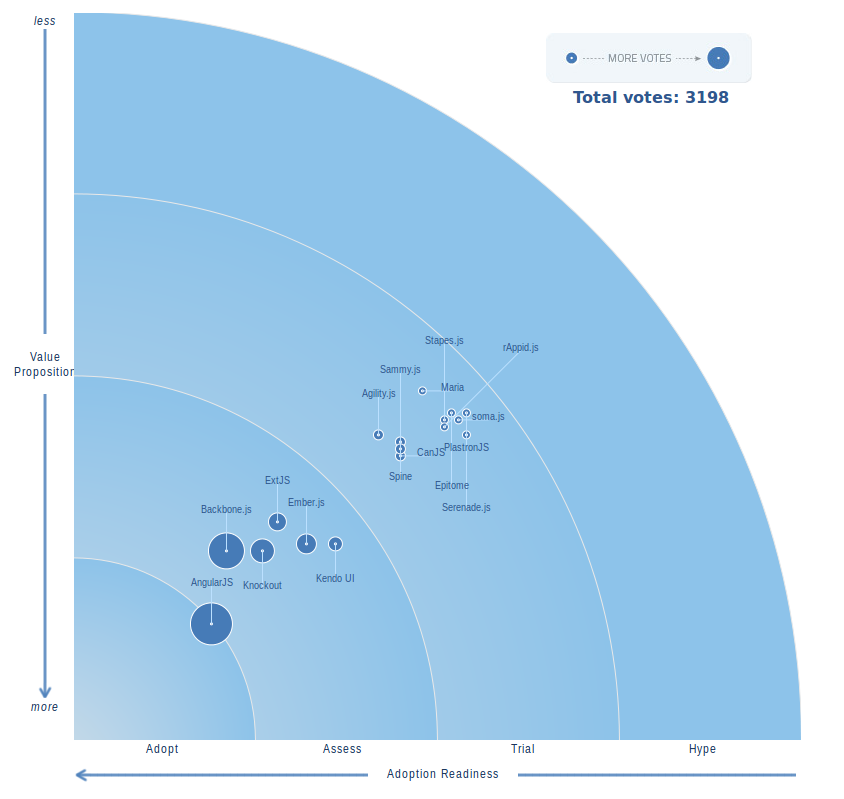
\includegraphics[scale=0.6]{images/angularjs_framework_comparison.png}
    \caption{Gráfico Comparando Frameworks Javascript.}
    \label{fig:Gráfico Comparando Frameworks Javascript}
    \end{figure}
    
Um projeto de AngularJS é formado por páginas HTML e arquivos Javascript em conjunto com as diretivas próprias do Angular. 

\subsubsection{SPA - Single Page Application}

O conceito de Single Page Application é  quando cada parte de página é carregada de forma independente, ou seja, quando uma página é carregada, todas as demais atualizações são feitas através de requisições AJAX\footnote{AJAX é uma metodologia que utiliza tecnologias como XML e Javascript para fazer requisições assíncronas ao servidor e com as informações retornadas modificar uma pagina carregada através de DOM sem necessidade de recarregar todo conteúdo da pagina.} e renderizações parciais na página.
    Através destas renderizaçoes parciais temos um aumento de performance devido a diminuição da quantidade de dados que precisam ser trafegadas entre o cliente e o servidor.

\subsubsection{Data Biding}

É recurso para facilitar o desenvolvimento do sistema enquanto o AngularJS manipula e cuida de atualizar as informações da pagina. Através do uso de alguns controles na pagina em HTML o AngularJS consegue identificar e mapear os atributos a serem atualizados.

\subsubsection{Injeção de dependências}

A injeção de dependências consiste basicamente  em fornecer recursos extras necessário na aplicação de forma transparente ao usuário, de modo que o desenvolvedor somente deverá solicitar um recurso, que será injetado pelo framework e ficará disponível para uso.

\subsection{Node.js}
O Node.js é uma plataforma de desenvolvimento web que funciona com a linguagem Javascript no lado do servidor, para criação de aplicações e páginas web de alta escalabilidade, sendo que foi concebida por  Ryan Dahl em 2009 \cite{appRealTime}, e desde então vem ganhando muita popularidade entre os desenvolvedores web, e sendo utilizado por grandes empresas e instituições tais como LinkedIn, Microsoft, GitHub, MySpace, entre outras\footnote{\url{https://github.com/joyent/node/wiki/Projects,-Applications,-and-Companies-Using-Node}}. A escolha da linguagem Javascript foi devido a enorme quantidade de bibliotecas para I/O que a linguagem possui, permitindo assim ao Ryan criar as funções assíncronas para a plataforma. 

A arquitetura do Node.js é composta em sua maior parte por componentes  desenvolvidos em C e em Javascript \cite{nodeInAction}, sendo que os principais componentes da parte escrita em C são: a  máquina virtual para Javascript do Google chamada V8, que é usada no projeto do Google Chrome, o Node Bindings\footnote{São códigos executáveis que fazem com que o V8 e a biblioteca em javascript padrão do node sejam capazes de se comunicar.}, a Thread Pool\footnote{}, e o Event Loop, e em relação a parte do Javascript, foi criada uma biblioteca chamada Node Standard Library, para permitir que o Node.js interprete códigos em Javascript.

%figura

    \begin{figure}[hb]
    \centering
    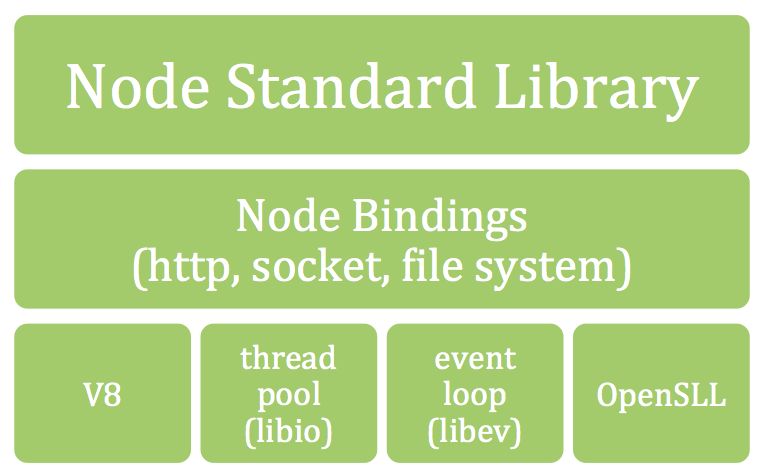
\includegraphics[scale=0.4]{images/node_platform.png}
    \caption{Arquitetura do Node.}
    \label{fig:Arquitetura do Node}
    \end{figure}
  
    
    O Node.js foi criado de forma que suas funcionalidades pudessem ser estendidas através de módulos, para implementar diversos componentes middleware que facilitem o desenvolvimento de aplicações web. Estes módulos são geralmente instalados através de um gerenciador de pacotes conhecido como npm\footnote{Node Package Manager.}, que facilita a compilação, instalação e atualização, e também gerencia as dependências.

\subsubsection{I/O não bloqueante e orientado a eventos}

Quando necessitamos acessar\footnote{Seja para leitura, escrita, atualização ou remoção.} os dados de uma aplicação, estes dados podem estar em vários locais, tais como na memória (L1, L2, RAM), no disco ou na rede, e cada local contem uma latência de I/O diferente, no caso para memória quando necessitamos acessar a L1 gastamos aproximadamente  3 ciclos, passando para 14 ciclos na L2 e para 250 ciclos na RAM, já para o disco e para a rede a quantidade de ciclos necessários tem um aumento significativo, sendo aproximadamente 41 e 250 milhões de ciclos, respectivamente, ou seja, quando utilizamos a memória podemos considerar que será um acesso rápido, também conhecido como não bloqueante, e já para o disco e a rede consideramos que será um acesso lento, também conhecido como bloqueante

O Node.js foi desenvolvido com base no conceito de “I/O não bloqueante”\cite{nodeRight}  (também conhecido por I/O assíncrono), e isto foi feito através da utilização de uma construção  de programação conhecida como  Event Loop, que é um laço infinito que para cada iteração faz uma verificação se existem novos eventos em uma fila de eventos, sendo que o Node.js é considerado uma aplicação Single Thread\footnote{Apesar de possuir uma Thread pool}. Um exemplo do funcionamento do Event Loop é quando se recebe uma requisição de um evento não bloqueante, sendo que este evento será tratado diretamente pela Thread principal, e outra situação é quando se recebe uma requisição bloqueante, como por exemplo uma leitura de disco, esta requisição então é enviada para a Thread Pool do Node.js, que irá criar uma thread para tratá-la, e quando terminar, a thread envia uma mensagem para a Thread principal que então executa a função de callback\footnote{} respectiva a requisição.

%figura
    \begin{figure}[h]
    \centering
    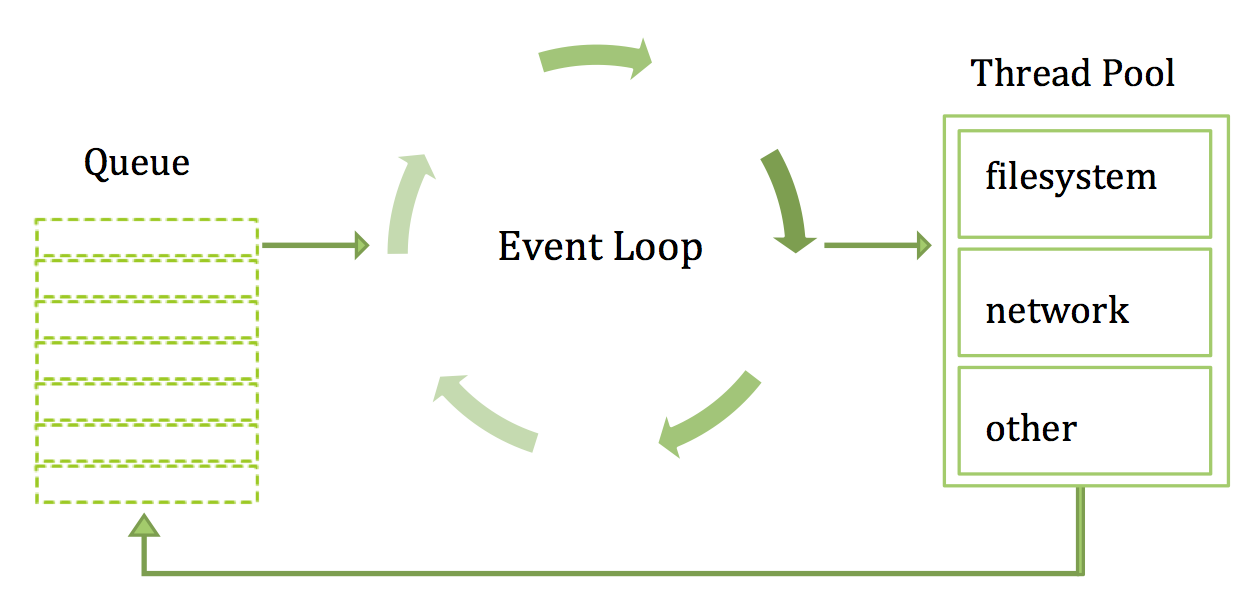
\includegraphics[scale=0.3]{images/node_event_loop.png}
    \caption{Event Loop do Node.js.}
    \label{fig:Event Loop do Node.js}
    \end{figure}
    
\section{Socket.IO}

O Socket.io é uma API em Javascript que permite que a comunicação entre o servidor e o cliente ocorra sem dificuldades e em tempo real. Ele abstrai e utiliza o protocolo WebSocket\footnote{É um protocolo orientado a eventos que permite abrir uma sessão de comunicação interativa entre o navegador do cliente e o sevidor, sendo possível enviar mensagens para um servidor e receber respostas sem ter que consultar o servidor para uma resposta.},  e também possui outras alternativos caso seja um ambiente que não suporte WebSocket.